\section{Experiments}
\label{sec:experiments}

We design experiments to answer four research questions. \textbf{RQ1:} How well can current coding agents implement repositories from fuzzy requirements (Section~\ref{sec:main-results})? \textbf{RQ2:} How much of the gap to GroundPRD can interaction recover (Section~\ref{sec:main-results})? \textbf{RQ3:} Where do bottlenecks arise in the clarification-to-implementation pipeline (Section~\ref{sec:analysis})? \textbf{RQ4:} How sensitive are results to the agent framework, User Agent backbone, interaction budget, test scaffolding, thinking configuration, execution environment, and implementation language (Section~\ref{sec:analysis})?

\subsection{Experimental Settings}
\label{sec:experimental-settings}

\paragraph{Datasets and metrics.}
We report the main comparison on the full \rcb{} benchmark and use \rcblite{}, a 50-repository subset selected by sorting the full tasks by golden-code LOC, for repeated ablations. The full split measures realistic repository-scale performance, while \rcblite{} enables controlled comparisons across model backbones, agent frameworks, User Agent backbones, interaction budgets, thinking-budget settings, and execution environments.

We use the functional, agentic, structural, and interaction metrics defined in Section~\ref{sec:metrics}; all reported values are percentages unless noted otherwise.

\paragraph{Models and execution.}
The main \rcblite{} and full \rcb{} comparisons evaluate six coding models under the Claude Code framework~\cite{anthropic_claude_agent_sdk_2026}: GPT-5.5~\cite{singh2025openai}, Claude-Opus-4.8~\cite{anthropic_claude_opus_4_8_2026}, Claude-Sonnet-4.6~\cite{anthropic_claude_sonnet_4_6_2026}, GLM-5.1~\cite{zeng2026glm}, Gemini-3.1-Pro~\cite{google_deepmind_gemini_3_1_pro_2026}, and MiniMax-M2.5~\cite{chen2026minimax}. Unless otherwise specified, the main result tables report the adaptive thinking setting, where the model decides its own thinking length. For GLM-5.1, we additionally analyze a think-8k setting that caps the maximum thinking length at 8k tokens. The tested agent receives a fuzzy PRD, may ask at most 16 questions, and interacts with a DeepSeek-V3.2 User Agent that routes questions to grounded hidden constraints rather than generating free-form answers. GroundPRD runs remove ambiguity by providing the complete requirement document upfront and therefore serve as an upper-bound reference. Although tasks are derived from real open-source repositories, the evaluated agents do not see original repository identities, original source code, original tests, or hidden implementation details; they see only benchmark-authored task materials and any clarification returned through grounded User Agent records.

\subsection{Main Results}
\label{sec:main-results}

The main results address two questions in sequence. To answer RQ1, we first evaluate the default Fuzzy L1 setting with User Agent interaction on the full benchmark. This baseline alone cannot separate missing requirements from weak implementation. To answer RQ2, we vary \emph{requirement exposure}---the amount and organization of requirement information available before coding---over the same tasks, from Fuzzy L1--L3 and RecoveredPRD to the complete GroundPRD.

Under the shared default framework and interaction protocol, Table~\ref{tab:main-results-full} compares six coding models on the full benchmark, while Table~\ref{tab:main-results-lite} reports the corresponding \rcblite{} results.

\begin{table*}[t]
\centering
\caption{Main results on the full \rcb{} split using Claude Code. Values are percentages; File and LOC are generated-to-golden ratios and may exceed 100.}
\label{tab:main-results-full}
\small
\begin{tabular}{lccccccc}
\toprule
\multirow{2}{*}{Model} & \multicolumn{4}{c}{Test Cases Pass Rate} & \multicolumn{3}{c}{Agentic Evaluation} \\
\cmidrule(lr){2-5}\cmidrule(lr){6-8}
 & Overall & Public & Native & Enhanced & Sem. & API & Design \\
\midrule
Claude-Opus-4.8 & \textbf{38.2} & 48.5 & 41.4 & \textbf{35.5} & 22.6 & \textbf{12.1} & \textbf{44.4} \\
GPT-5.5 & 37.2 & \textbf{50.3} & \textbf{42.0} & 32.8 & 21.5 & 9.3 & 36.5 \\
Gemini-3.1-Pro & 27.0 & 37.0 & 30.7 & 23.5 & 18.9 & 8.9 & 28.6 \\
GLM-5.1 & 26.6 & 36.8 & 30.0 & 23.7 & 21.1 & 10.0 & 37.1 \\
Claude-Sonnet-4.6 & 21.8 & 29.0 & 24.1 & 19.4 & \textbf{22.9} & 10.1 & 37.5 \\
MiniMax-M2.5 & 0.8 & 1.5 & 1.2 & 0.6 & 11.8 & 5.5 & 23.1 \\
\midrule
\multirow{2}{*}{Model} & \multicolumn{4}{c}{Structural Assessment} & \multicolumn{3}{c}{Interaction Quality} \\
\cmidrule(lr){2-5}\cmidrule(lr){6-8}
 & File & LOC & Class & Method & Constr. & Fallback & Budget \\
\midrule
Claude-Opus-4.8 & 337.6 & 981.1 & \textbf{17.5} & \textbf{10.8} & 69.6 & 21.6 & 81.5 \\
GPT-5.5 & 44.0 & 154.9 & 14.6 & 9.0 & \textbf{73.7} & \textbf{20.4} & 76.8 \\
Gemini-3.1-Pro & 46.2 & 221.9 & 15.9 & 10.4 & 56.3 & 28.1 & 74.2 \\
GLM-5.1 & 12.1 & 15.9 & 15.0 & 9.6 & 63.9 & 28.1 & 95.0 \\
Claude-Sonnet-4.6 & 15.5 & 15.9 & 17.0 & 10.4 & 57.7 & 24.2 & 76.0 \\
MiniMax-M2.5 & 41.2 & 117.0 & 13.1 & 7.5 & 44.3 & 28.5 & 70.6 \\
\bottomrule
\end{tabular}
\end{table*}

\begin{table*}[htbp]
\centering
\caption{Main results on \rcblite{} using Claude Code. Values are percentages; File and LOC are generated-to-golden ratios and may exceed 100.}
\label{tab:main-results-lite}
\small
\begin{tabular}{lccccccc}
\toprule
\multirow{2}{*}{Model} & \multicolumn{4}{c}{Test Cases Pass Rate} & \multicolumn{3}{c}{Agentic Evaluation} \\
\cmidrule(lr){2-5}\cmidrule(lr){6-8}
 & Overall & Public & Native & Enhanced & Sem. & API & Design \\
\midrule
Claude-Opus-4.8 & 48.2 & 56.6 & 52.9 & 44.4 & 28.5 & 14.3 & \textbf{49.1} \\
GPT-5.5 & \textbf{53.3} & \textbf{63.8} & \textbf{60.9} & \textbf{47.4} & 30.0 & 15.2 & 48.7 \\
Gemini-3.1-Pro & 36.6 & 45.5 & 41.4 & 33.1 & 27.2 & 14.2 & 31.4 \\
GLM-5.1 & 40.0 & 47.6 & 44.5 & 35.9 & 22.6 & 11.0 & 37.9 \\
Claude-Sonnet-4.6 & 40.2 & 47.0 & 44.1 & 37.1 & \textbf{34.2} & \textbf{16.1} & 44.3 \\
MiniMax-M2.5 & 2.8 & 2.7 & 4.4 & 1.9 & 19.2 & 8.2 & 28.6 \\
\midrule
\multirow{2}{*}{Model} & \multicolumn{4}{c}{Structural Assessment} & \multicolumn{3}{c}{Interaction Quality} \\
\cmidrule(lr){2-5}\cmidrule(lr){6-8}
 & File & LOC & Class & Method & Constr. & Fallback & Budget \\
\midrule
Claude-Opus-4.8 & 45.3 & 47.1 & \textbf{36.8} & 17.7 & 67.8 & \textbf{17.9} & 75.5 \\
GPT-5.5 & 36.8 & 35.0 & 32.6 & 17.7 & \textbf{73.2} & 21.0 & 71.7 \\
Gemini-3.1-Pro & 62.2 & 743.3 & 35.4 & 18.0 & 58.0 & 23.5 & 68.5 \\
GLM-5.1 & 32.4 & 64.5 & 33.2 & 17.4 & 63.3 & 28.4 & 95.4 \\
Claude-Sonnet-4.6 & 33.9 & 51.0 & 34.9 & \textbf{18.4} & 60.8 & 25.9 & 75.1 \\
MiniMax-M2.5 & 17.9 & 32.5 & 30.8 & 12.6 & 48.1 & 28.1 & 69.1 \\
\bottomrule
\end{tabular}
\end{table*}

Table~\ref{tab:language-results-full} reports the balanced programming-language breakdown. The four metric families expose distinct capabilities. Functionally, Public rates consistently exceed Enhanced rates, indicating difficulty beyond visible examples. Agentic scores do not mirror the functional ranking: Claude-Sonnet-4.6 has the highest semantic score but ranks fifth in Overall. Structural ratios reveal sharply different construction strategies; Claude-Opus-4.8 produces much larger repositories than GPT-5.5, despite their similar Overall rates. Interaction metrics show a further separation: GPT-5.5 recovers more constraints than Claude-Opus-4.8 yet scores one point lower Overall. Neither repository scale nor recovered information is therefore a proxy for correctness.

\begin{table}[t]
\centering
\caption{Per-language overall pass rate on the full \rcb{} split.}
\label{tab:language-results-full}
\small
\begin{adjustbox}{width=\linewidth, center}
\begin{tabular}{lcccccc}
\toprule
Model & C\# & C++ & Dart & Go & Java & JavaScript \\
\midrule
Claude-Opus-4.8 & 39.9 & 29.5 & 38.7 & 44.8 & 39.1 & 34.4 \\
GPT-5.5 & 39.4 & 31.5 & 40.6 & 39.7 & 38.4 & 34.9 \\
Gemini-3.1-Pro & 18.6 & 13.8 & 26.7 & 22.0 & 35.0 & 33.2 \\
GLM-5.1 & 23.2 & 26.3 & 33.4 & 21.9 & 20.8 & 27.6 \\
Claude-Sonnet-4.6 & 23.6 & 19.1 & 21.9 & 30.1 & 19.3 & 18.9 \\
MiniMax-M2.5 & 0.0 & 1.0 & 0.9 & 0.1 & 0.0 & 0.2 \\
\midrule
Model & Kotlin & PHP & Python & Ruby & Rust & TypeScript \\
\midrule
Claude-Opus-4.8 & 39.3 & 36.5 & 33.0 & 38.9 & 40.3 & 43.7 \\
GPT-5.5 & 31.7 & 42.2 & 34.9 & 41.4 & 37.4 & 34.6 \\
Gemini-3.1-Pro & 26.8 & 35.9 & 31.4 & 24.9 & 22.7 & 32.7 \\
GLM-5.1 & 29.9 & 38.4 & 26.8 & 19.4 & 23.9 & 27.3 \\
Claude-Sonnet-4.6 & 22.7 & 24.1 & 23.6 & 15.7 & 21.4 & 20.5 \\
MiniMax-M2.5 & 2.1 & 0.2 & 4.5 & 0.3 & 0.0 & 0.9 \\
\bottomrule
\end{tabular}
\end{adjustbox}
\end{table}

\textbf{Answer to RQ1.} Current agents implement a nontrivial fraction of fuzzy requirements, but the best Overall rate is only 38.2\%. The leading model varies across programming languages, and similar functional scores conceal substantial differences in artifact design, repository scale, and requirement recovery. The consistent Public--Enhanced gap further shows that reproducing visible examples does not ensure robust behavior.

Figure~\ref{fig:prd-levels-plot} compares three fuzzy levels, RecoveredPRD, and GroundPRD over the same tasks. RecoveredPRD is constructed by appending all L1 question--answer records to the Fuzzy L1 PRD before generation, thereby removing retrieval while preserving their fragmented form. L2 restores selected L1 ambiguity points, L3 retains most of GroundPRD, and GroundPRD provides the complete coherent specification. Their semantic alignment is validated in Section~\ref{sec:artifact-verification}; Figure~\ref{fig:prd-token-comparison} quantifies L1--L3 exposure.

\begin{figure}[t]
\centering
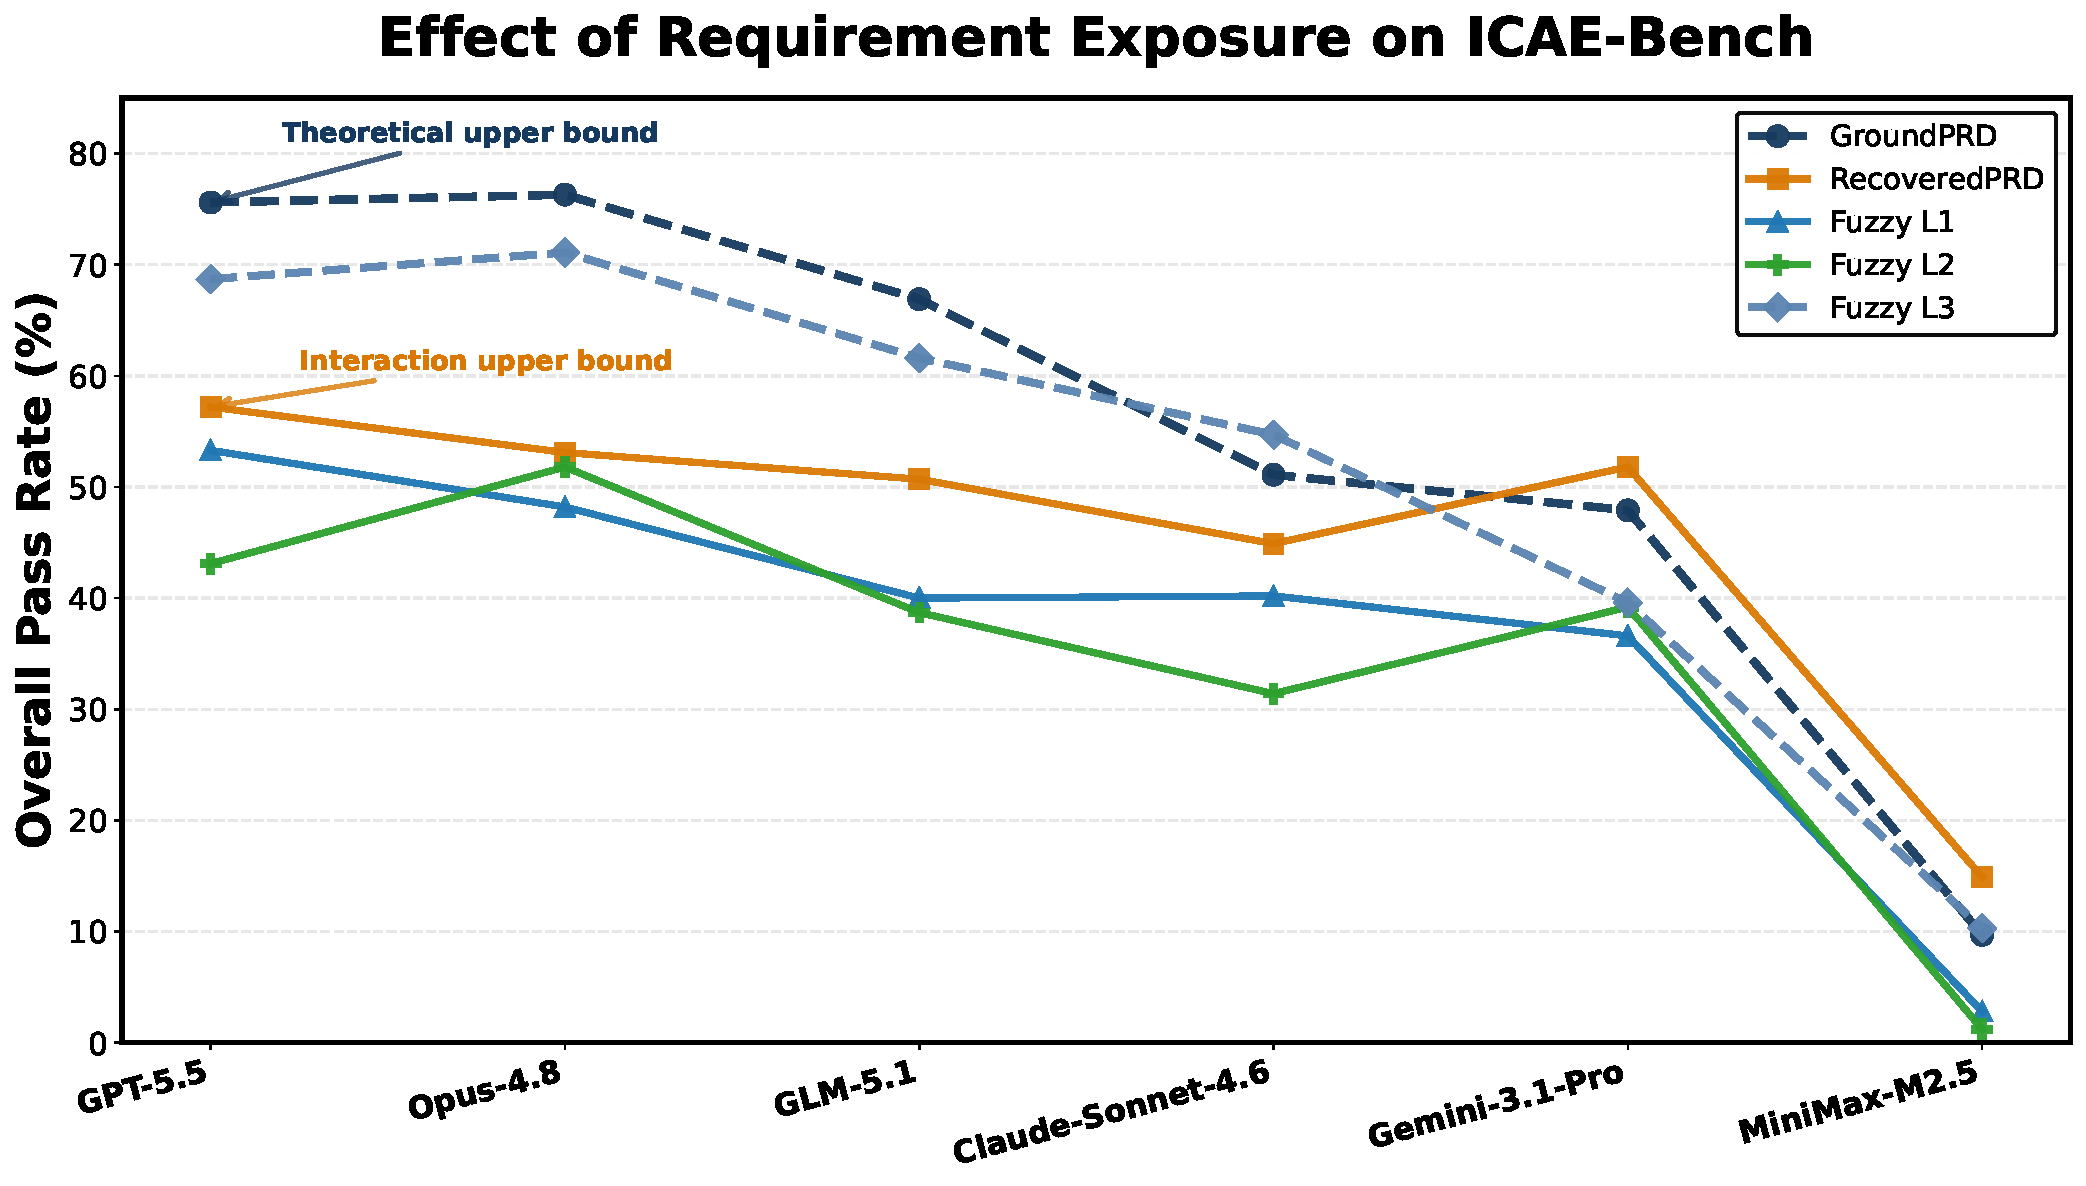
\includegraphics[width=\linewidth]{figures/prd_levels_comparison.pdf}
\caption{Overall pass rate across PRD ambiguity settings on \rcblite{}. Fuzzy L2 restores a subset of the ambiguity points hidden in L1; Fuzzy L3 preserves more of GroundPRD through limited deletion and light ambiguity-oriented rewriting.}
\label{fig:prd-levels-plot}
\end{figure}

\begin{figure}[htbp]
\centering
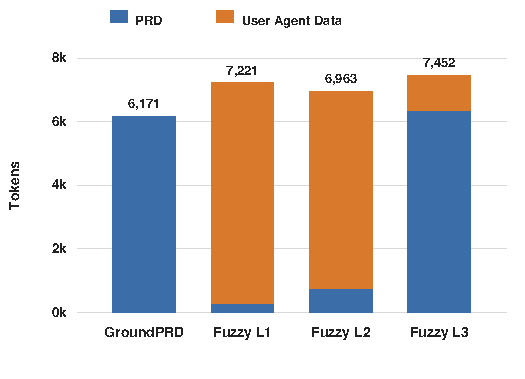
\includegraphics[width=\linewidth]{figures/requirement_token_composition.pdf}
\caption{Requirement-token comparison on \rcblite{}. User Agent Data is accessible only through interaction.}
\label{fig:prd-token-comparison}
\end{figure}

GroundPRD performs best for four of six models. RecoveredPRD remains below it for GPT-5.5, Claude-Opus-4.8, GLM-5.1, and Claude-Sonnet-4.6, despite exposing every recoverable L1 record. Gemini-3.1-Pro and MiniMax-M2.5 are exceptions, and the fuzzy-level trends are not uniformly monotonic. Thus, retrieval explains only part of the gap: agents must also organize fragmented answers, retain them, and convert them into implementation decisions. Figure~\ref{fig:ambiguity-category-distribution} confirms that this challenge spans multiple ambiguity categories rather than one missing-information type.

\begin{figure}[t]
\centering
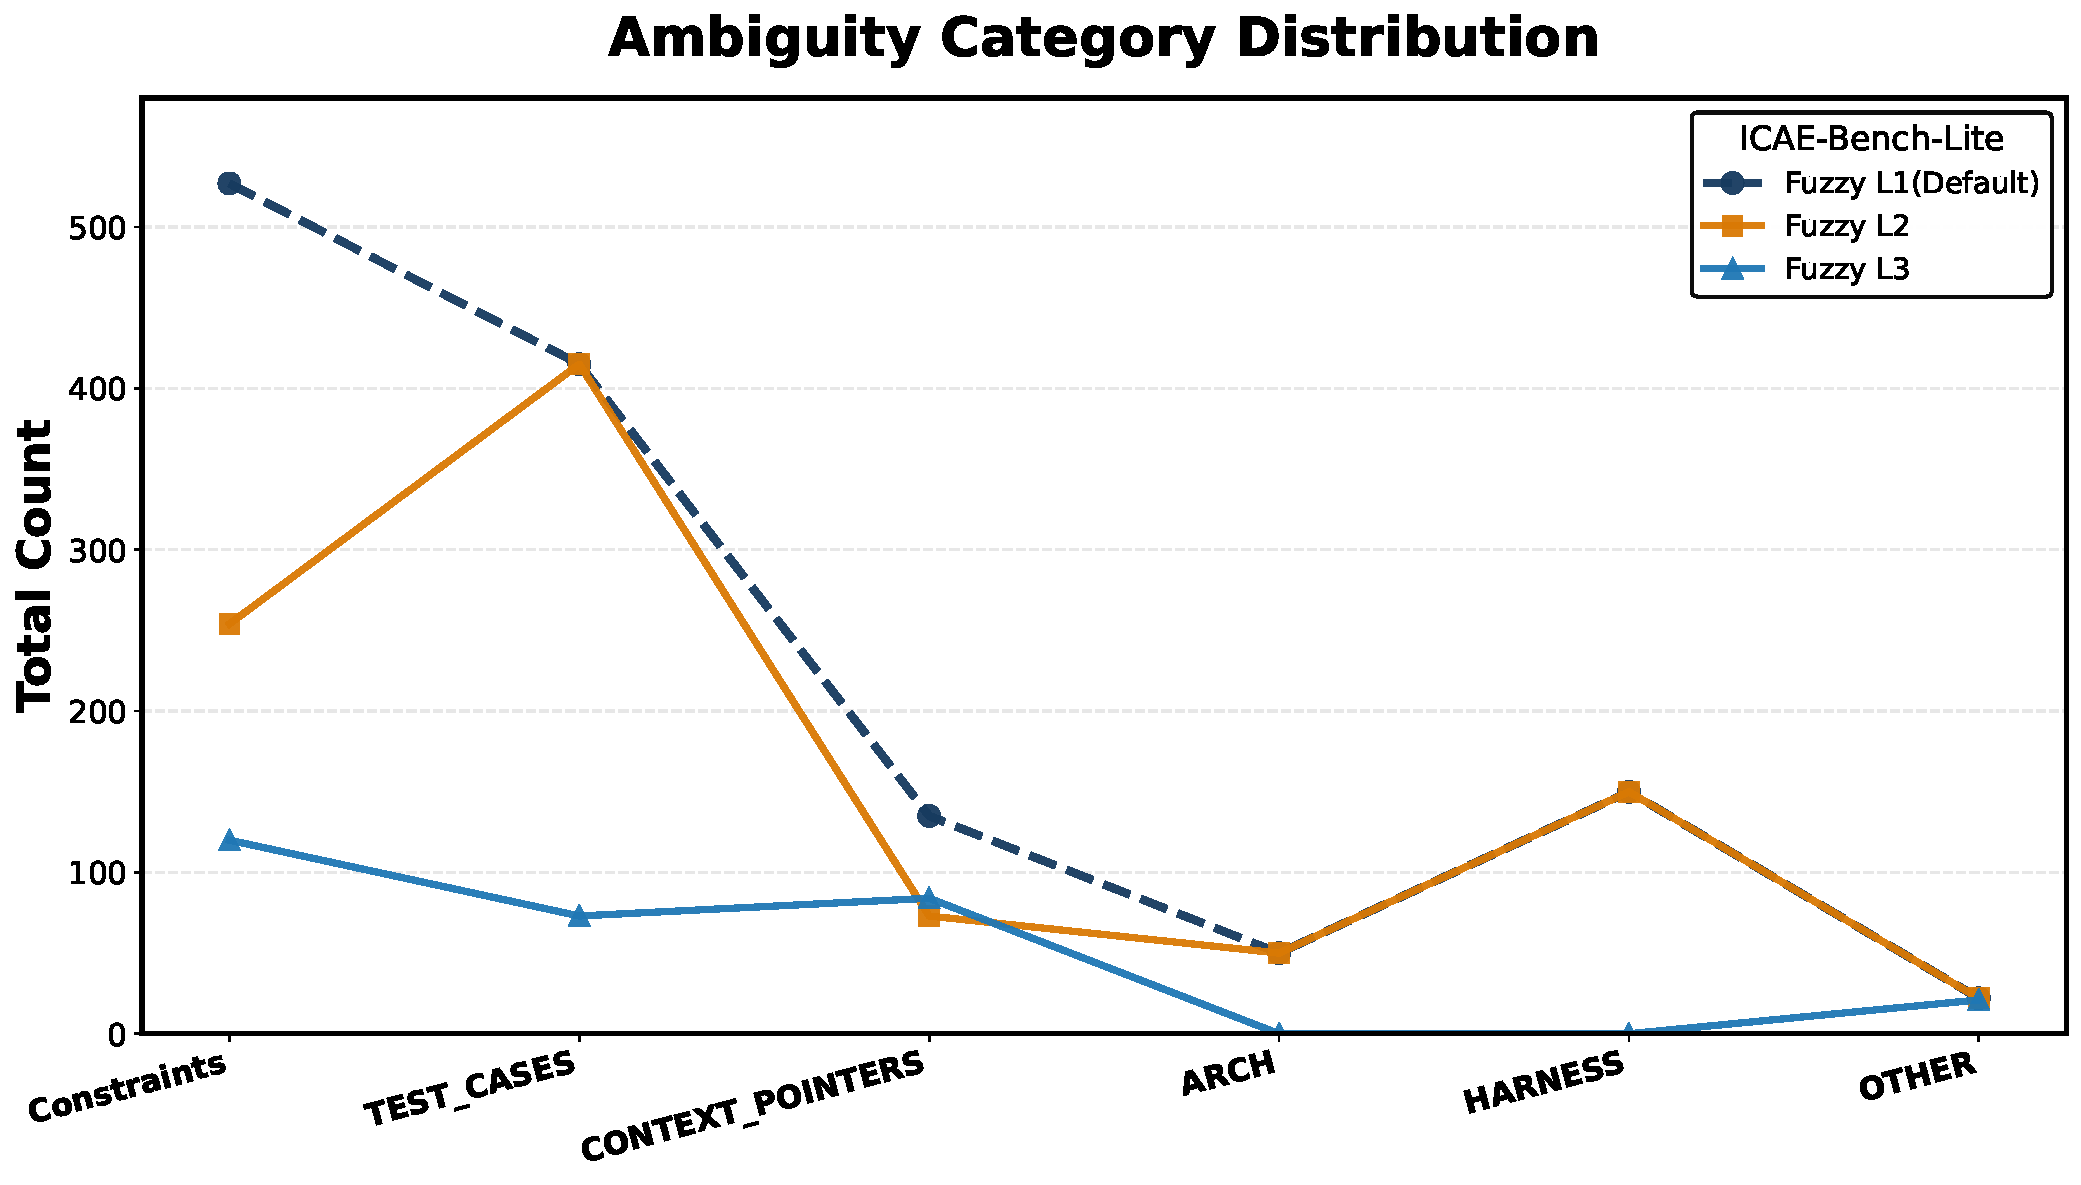
\includegraphics[width=\linewidth]{figures/category_lines_comparison.pdf}
\caption{Distribution of ambiguity categories across Fuzzy L1--L3 in \rcb{}.}
\label{fig:ambiguity-category-distribution}
\end{figure}

\textbf{Answer to RQ2.} Interaction and greater initial exposure recover only part of the gap to GroundPRD, with substantial variation across models. Even complete access to recoverable records is insufficient when those records are not organized and used effectively during implementation.

Together, RQ1 and RQ2 expose two distinct gaps. The \emph{requirement-access gap} separates a fuzzy PRD from the information recoverable through clarification; the \emph{information-to-execution gap} separates recovered requirements from a correct repository. The first motivates interaction, whereas the second concerns retention, implementation, and verification over a long development trajectory. The following analyses focus on where this second gap emerges and which components can reduce it.


\subsection{Analysis}
\label{sec:analysis}

The main results show that additional requirement information recovers only part of the performance gap. To answer RQ3, evaluator-visible failure categories localize breakdowns, while a controlled executable-feedback intervention tests whether verification reduces them. We then answer RQ4 by varying the interaction stack, reasoning configuration, and execution setting.

\subsubsection{Failure Mode Taxonomy}
\label{sec:failure-modes}

Pass rate alone cannot locate a breakdown. Figure~\ref{fig:failure-modes} therefore reports four evaluator-visible failure modes. \emph{Mismatch} means that a case produced output that differed from the expected result, indicating a logic or behavioral-correctness failure. \emph{Missing} means that some cases produced no output while the suite otherwise ran, indicating incomplete feature coverage. \emph{Exec.} means that the harness ran but all outputs were absent because of a recognized build or runtime error, indicating buildability, dependency, or environment failure. \emph{No Test} means that the agent did not produce the required \texttt{rcb\_tests/test.sh} entry point, indicating instruction-following or harness-compliance failure.

Failure labels are assigned per Public, Native, and Enhanced suite. A repository may therefore exhibit different modes across suites, and a single suite may contain both missing and mismatched cases; the columns are not mutually exclusive. A \emph{Clean} repository passes every evaluated case. We omit this success category from the failure-mode figure; only 1--13 of 480 repositories per model are Clean because this repository-level criterion is stricter than the case-level Overall pass rate. Constraint forgetting and interaction inefficiency are not directly identifiable from execution outcomes and are analyzed through interaction metrics and controlled ablations.

\begin{figure}[htbp]
\centering
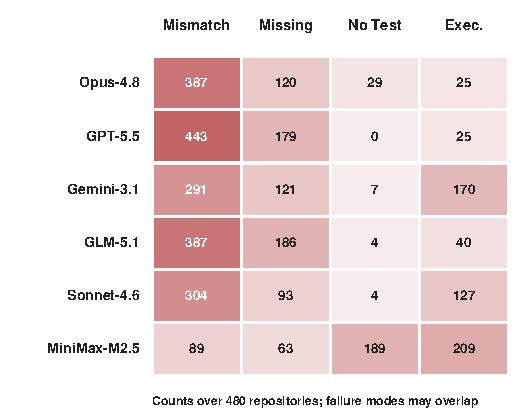
\includegraphics[width=\linewidth]{figures/failure_modes_heatmap.pdf}
\caption{Evaluator-visible outcomes on full \rcb{} main runs. Failure modes are not mutually exclusive.}
\label{fig:failure-modes}
\end{figure}

The counts expose distinct bottlenecks. Stronger models more often reach execution but violate the behavioral contract, whereas weaker models more often omit the harness or fail during execution. Missing outputs further isolate incomplete feature coverage from incorrect implemented behavior.

\subsubsection{Effect of Test Scaffolding}
\label{sec:test-scaffolding}

Failure categories do not reveal whether clarified information is difficult to apply and verify. We therefore provide ready-to-run Public case files while keeping the same case content recoverable through the User Agent in both settings. Overall rises from 37.4\% to 61.8\%, while constraint coverage changes from 63.8\% to 61.2\% (Table~\ref{tab:test-scaffold}).

\begin{table}[t]
\centering
\caption{Effect of placing Public case files in the workspace for GLM-5.1 think-8k on \rcblite{}. \textbf{w/} includes the files; \textbf{w/o} (default) omits them while retaining interaction-based access to the same case content.}
\label{tab:test-scaffold}
\small
% \begin{adjustbox}{width=\linewidth, center}
\begin{tabular}{lcccc}
\toprule
Setting & Pass OA & Design & Constr. & Fallback \\
\midrule
w/ & \textbf{61.8} & 38.5 & 61.2 & 29.7 \\
w/o (default) & 37.4 & \textbf{43.2} & \textbf{63.8} & \textbf{27.7} \\
\bottomrule
\end{tabular}
% \end{adjustbox}
\end{table}

The treatment changes the representation and actionability of information, not its semantic coverage. Public files package inputs, expected outputs, and the invocation format as an executable structure; without them, the agent must recover fragments through questions and reconstruct the same verification scaffold. Immediate execution and debugging feedback therefore explain the gain more directly than additional requirements. The improvement also extends to Native and Enhanced behavior despite slightly lower constraint coverage.

\textbf{Answer to RQ3.} The analyses in Sections~\ref{sec:failure-modes} and~\ref{sec:test-scaffolding} locate breakdowns at both execution and behavioral fidelity and show that verification can improve correctness without recovering more constraints. Low scores therefore reflect failures across the clarification-to-implementation chain rather than requirement access alone.


% We organize the controlled factors into the interaction stack, thinking configuration, and execution environment.

\subsubsection{Impact of Agent Frameworks}
\label{sec:framework}

RQ3 shows that obtaining requirements is not enough; the surrounding framework may determine whether they survive implementation. Because frameworks control editing, execution, and state tracking, Table~\ref{tab:framework} tests the same models and tasks under Claude Code and OpenHands~\cite{wang2025openhands}. OpenHands lowers Overall for every model by 5.5--21.8 points, although GPT-5.5 recovers more constraints.

\begin{table}[t]
\centering
\caption{Agent-framework comparison on \rcblite{}.}
\label{tab:framework}
\small
\begin{adjustbox}{width=\linewidth, center}
\begin{tabular}{lcccc}
\toprule
Model & Pass OA & Design & Constr. & Fallback \\
\midrule
% --- 分组 1: Claude Code ---
\multicolumn{5}{c}{\textbf{\textit{Claude Code}}} \\
\midrule
GPT-5.5 & \textbf{53.3} & 48.7 & 73.2 & 21.0 \\
Claude-Opus-4.8 & 48.2 & 49.1 & 67.8 & 17.9 \\
Claude-Sonnet-4.6 & 40.2 & 44.3 & 60.8 & 25.9 \\
GLM-5.1 & 37.4 & 43.2 & 63.8 & 27.7 \\
Gemini-3.1-Pro & 36.6 & 31.4 & 58.0 & 23.5 \\
MiniMax-M2.5 & 2.8 & 28.6 & 48.1 & 28.1 \\
\midrule
% --- 分组 2: OpenHands ---
\multicolumn{5}{c}{\textbf{\textit{OpenHands}}} \\
\midrule
GPT-5.5 & 31.5 & 39.4 & \textbf{76.8} & 20.0 \\
Claude-Opus-4.8 & 42.7 & \textbf{56.6} & 68.6 & \textbf{13.1} \\
Claude-Sonnet-4.6 & 23.6 & 44.3 & 55.5 & 15.2 \\
GLM-5.1 & 28.4 & 43.1 & 72.0 & 24.3 \\
Gemini-3.1-Pro & 28.6 & 34.8 & 62.2 & 25.9 \\
MiniMax-M2.5 & 1.1 & 31.7 & 43.0 & 27.6 \\
\bottomrule
\end{tabular}
\end{adjustbox}
\end{table}

Framework sensitivity is model dependent. GPT-5.5, the strongest model under Claude Code, drops by 21.8 points and falls behind Claude-Opus-4.8 under OpenHands; Claude-Opus-4.8 drops by only 5.5 points. Thus, framework choice changes both absolute performance and ranking. GPT-5.5's higher OpenHands constraint coverage does not offset weaker downstream execution, underscoring the role of reliable editing, command execution, state tracking, and termination.

\subsubsection{Impact of User Agent Capability}
\label{sec:user-agent-capability}

The framework comparison changes the coding scaffold, but clarification quality may also depend on the model acting as the User Agent. We therefore change only the User Agent's base model while keeping its prompt, grounded records, coding model, tasks, and query budget fixed. Table~\ref{tab:user-agent-ablation} compares three base models under both GLM-5.1 thinking configurations.

\begin{table}[t]
\centering
\caption{User Agent backbone ablation on \rcblite{} with GLM-5.1.}
\label{tab:user-agent-ablation}
\small
\begin{adjustbox}{width=\linewidth, center}
\begin{tabular}{lcccc}
\toprule
User Agent & Pass OA & Constr. & Fallback & Budget \\
\midrule
\multicolumn{5}{c}{\textbf{\textit{Think-8k}}} \\
\midrule
Gemini-3.1-Flash-Lite & 27.4 & 75.2 & \textbf{24.5} & 92.1 \\
Gemini-3.5-Flash & \textbf{40.7} & 64.4 & 27.5 & 95.8 \\
DeepSeek-V3.2 & 37.4 & 63.8 & 27.7 & \textbf{89.8} \\
\midrule
\multicolumn{5}{c}{\textbf{\textit{Adaptive}}} \\
\midrule
Gemini-3.1-Flash-Lite & 33.2 & \textbf{75.8} & 26.8 & 95.0 \\
Gemini-3.5-Flash & 40.3 & 68.6 & 30.1 & 94.9 \\
DeepSeek-V3.2 & 40.0 & 63.3 & 28.4 & 95.4 \\
\bottomrule
\end{tabular}
\end{adjustbox}
\end{table}

The base model changes which records are retrieved but not correctness monotonically. Gemini-3.1-Flash-Lite attains the highest constraint coverage in both settings yet the lowest Overall, whereas Gemini-3.5-Flash and DeepSeek-V3.2 produce similar correctness with lower coverage. Once responses are restricted to grounded records, retrieving more constraints is therefore insufficient to improve the final repository.

\subsubsection{Impact of Interaction Budgets}
\label{sec:budget}

Even with a fixed User Agent, the agent may have too few opportunities to resolve ambiguity; conversely, more opportunities need not improve implementation. We therefore vary only the query budget for GLM-5.1 think-8k. Figure~\ref{fig:budget} shows Overall rates of 22.9\%, 37.4\%, and 34.4\% at budgets 8, 16, and 24, while coverage rises from 57.9\% to 71.4\%.

% \begin{table}[t]
% \centering
% \caption{Interaction-budget ablation on \rcblite{} with GLM-5.1 think-8k.}
% \label{tab:budget}
% \small
% \begin{adjustbox}{width=0.8\linewidth, center}
% \begin{tabular}{ccccc}
% \toprule
% Budget & Pass OA & Constr. & Fallback & Budget Use \\
% \midrule
% 8 & 22.9 & 57.9 & \textbf{18.8} & 99.0 \\
% 16 & \textbf{37.4} & 63.8 & 27.7 & 89.8 \\
% 24 & 34.4 & \textbf{71.4} & 31.9 & \textbf{85.6} \\
% \bottomrule
% \end{tabular}
% \end{adjustbox}
% \end{table}


\begin{figure}[!ht]
\centering
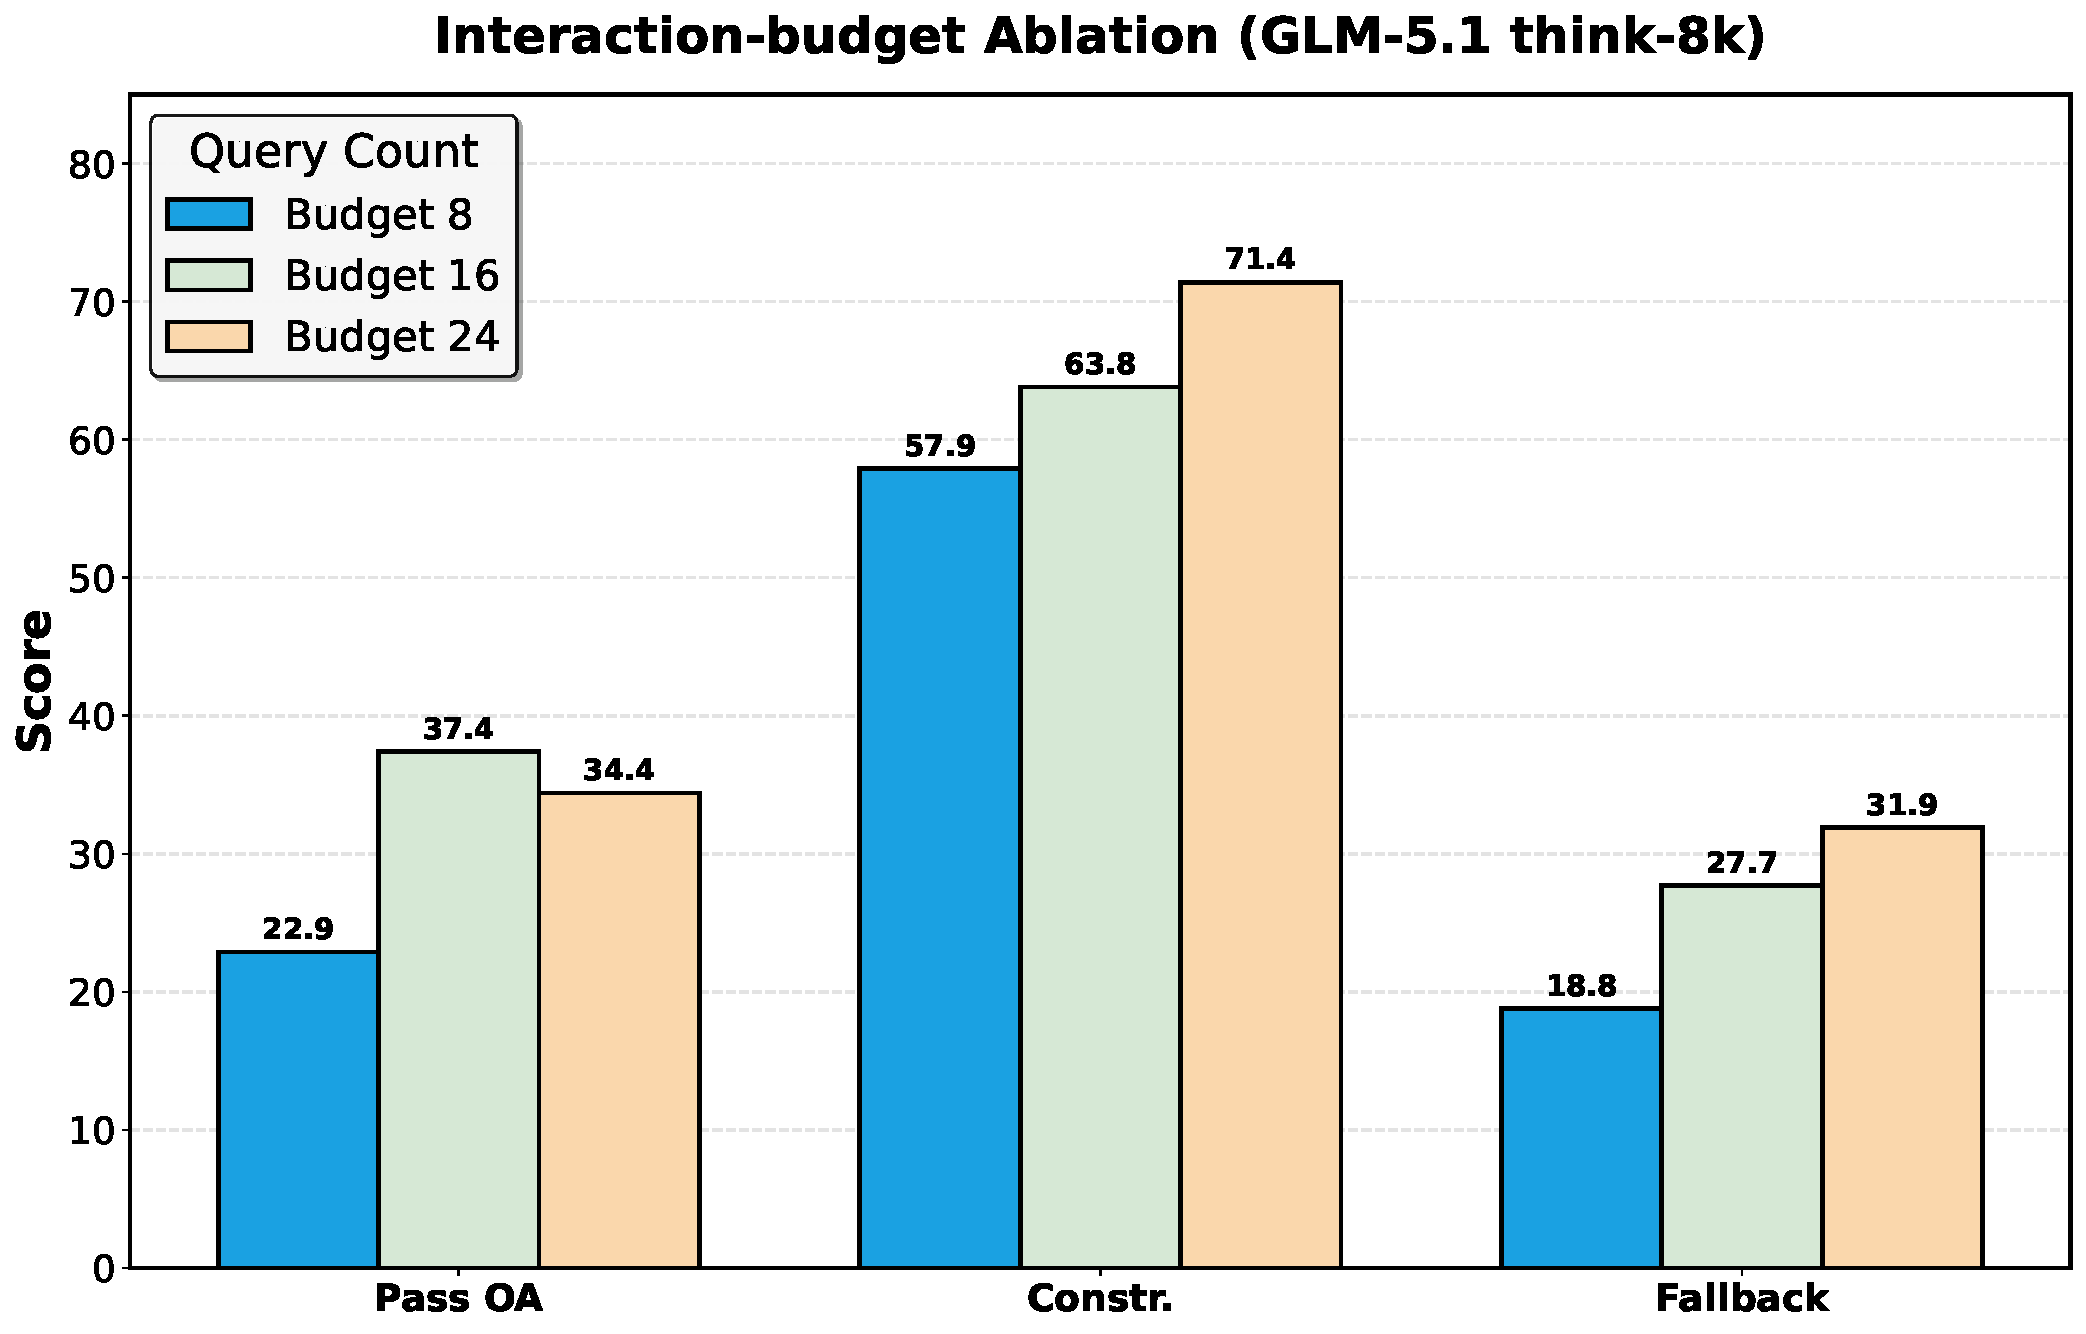
\includegraphics[width=\linewidth]{figures/budget_ablation.pdf}
\caption{Interaction-budget ablation on \rcblite{} with GLM-5.1 think-8k.}
\label{fig:budget}
\end{figure}

Fuzzy L1 contains slightly more than 20 ambiguity points per task on average (Figure~\ref{fig:ambiguity-category-distribution}), and one response can return up to three matched points. Sixteen queries therefore provide sufficient nominal retrieval capacity. Increasing the budget to 24 raises coverage but also raises fallback from 27.7\% to 31.9\%, while Overall falls from 37.4\% to 34.4\%. Once query capacity is no longer the main constraint, additional turns increasingly yield unmatched or redundant information and add integration burden rather than correctness.


\subsubsection{Impact of Thinking Configuration}
\label{sec:thinking}

The budget ablation motivates whether stronger deliberation helps use available information. We test two aspects of thinking: availability for Gemini-3.1-Pro and budget allocation for GLM-5.1. Enabling thinking raises Gemini-3.1-Pro from 26.7\% to 36.6\% Overall (Table~\ref{tab:thinking}); adaptive allocation raises GLM-5.1 from 37.4\% under think-8k to 40.0\% (Table~\ref{tab:glm-adaptive-think8k}). Deliberation benefits both comparisons, with a larger effect when thinking is enabled rather than disabled.

\begin{table}[t]
\centering
\caption{Thinking-mode ablation for Gemini-3.1-Pro on \rcblite{}.}
\label{tab:thinking}
\small
\begin{adjustbox}{width=\linewidth, center}
\begin{tabular}{lcccc}
\toprule
Setting & Overall & Public & Native & Enhanced \\
\midrule
Disabled & 26.7 & 33.6 & 29.6 & 24.3 \\
Enabled (default) & \textbf{36.6} & \textbf{45.5} & \textbf{41.4} & \textbf{33.1} \\
\bottomrule
\end{tabular}
\end{adjustbox}
\end{table}

\begin{table}[t]
\centering
\caption{GLM-5.1 adaptive vs.\ think-8k on \rcblite{}.}
\label{tab:glm-adaptive-think8k}
\small
\begin{adjustbox}{width=\linewidth, center}
\begin{tabular}{lcccc}
\toprule
Thinking Setting & Pass OA & Design & Constr. & Fallback \\
\midrule
Think-8k & 37.4 & \textbf{43.2} & \textbf{63.8} & \textbf{27.7} \\
Adaptive (default) & \textbf{40.0} & 37.9 & 63.3 & 28.4 \\
\bottomrule
\end{tabular}
\end{adjustbox}
\end{table}

\subsubsection{Impact of Execution Environment}
\label{sec:execution-environment}

Reasoning is only one part of repository construction; dependency availability also changes the available implementation space. We therefore compare both images using GLM-5.1 think-8k on \rcblite{}. The richer ultimate image lowers Overall from 37.4\% to 28.4\% while increasing constraint coverage and expanding generated repositories to 191.0\% of golden file count and 674.1\% of golden LOC (Table~\ref{tab:environment}).

\begin{table}[t]
\centering
\caption{Execution-environment comparison for GLM-5.1 think-8k on \rcblite{}.}
\label{tab:environment}
\small
\begin{adjustbox}{width=\linewidth, center}
\begin{tabular}{lccccc}
\toprule
Environment & Pass OA & Public Pass & File \% & LOC \% & Constr. \\
\midrule
Base image & \textbf{37.4} & \textbf{45.5} & 37.9 & 48.9 & 63.8 \\
Ultimate image & 28.4 & 38.8 & 191.0 & 674.1 & \textbf{69.1} \\
\bottomrule
\end{tabular}
\end{adjustbox}
\end{table}

More available components do not earn partial credit: each case must produce the expected output, while every added dependency, interface, or module introduces another failure point. The base image favors simpler, more self-contained implementations; the provisioned image permits more complex designs, as reflected by the size increase. Under a fixed reasoning budget, this broader action space also disperses implementation and verification effort. The results therefore associate richer provisioning with over-expansion rather than improved correctness; they do not imply that dependency availability is intrinsically harmful.

\subsubsection{Cross-lingual Generalization}
\label{sec:cross-lingual}

Finally, language-agnostic tests let us separate task semantics from implementation language. Reimplementing non-Python tasks in Python changes Overall from 26.6\% to 29.9\%, with mixed language-specific effects (Table~\ref{tab:cross-language-glm51}). Cross-language implementation is therefore feasible, but its benefit depends on the source task rather than following a uniform Python advantage.

\begin{table}[t]
\centering
\caption{Cross-language Overall pass rates for GLM-5.1 on \rcb{}.}
\label{tab:cross-language-glm51}
\small
\begin{adjustbox}{width=\linewidth, center}
\begin{tabular}{lcccccc}
\toprule
Implementation & \multicolumn{6}{c}{Original Language} \\
\cmidrule(lr){2-7}
 & C\# & C++ & Dart & Go & Java & JavaScript \\
\midrule
Original & 23.2 & 26.3 & 33.4 & 21.9 & 20.8 & 27.6 \\
Python & 26.4 \textcolor{green}{+3.2} & 43.6 \textcolor{green}{+17.3} & 39.6 \textcolor{green}{+6.2} & 25.8 \textcolor{green}{+3.9} & 30.3 \textcolor{green}{+9.5} & 29.3 \textcolor{green}{+1.7} \\
\midrule
Implementation & \multicolumn{6}{c}{Original Language} \\
\cmidrule(lr){2-7}
 & Kotlin & PHP & Ruby & Rust & TypeScript & Overall \\
\midrule
Original & 29.9 & 38.4 & 19.4 & 23.9 & 27.3 & 26.6 \\
Python & 27.5 \textcolor{red}{-2.4} & 23.8 \textcolor{red}{-14.6} & 27.2 \textcolor{green}{+7.8} & 26.6 \textcolor{green}{+2.7} & 35.6 \textcolor{green}{+8.3} & 29.9 \textcolor{green}{+3.3} \\
\bottomrule
\end{tabular}
\end{adjustbox}
\end{table}

\textbf{Answer to RQ4.} Framework support, executable Public scaffolding, and thinking materially improve correctness because they support implementation or verification. By contrast, higher constraint retrieval, larger interaction budgets, richer environments, and language changes are non-monotonic. These controlled comparisons show that configurations matter chiefly when they make requirement information actionable and verifiable, rather than merely increasing its availability.


\section{Discussion}
\label{sec:discussion}
Across RQ2--RQ4, access to more requirement information does not consistently yield more correct repositories. The strongest gains instead arise when information becomes actionable, as with executable Public cases. This pattern motivates agents that preserve clarified constraints, connect them to implementation decisions, and verify those decisions throughout repository construction.

\subsection{Validity of ICAE-Bench-Lite.}
The Overall rankings in Tables~\ref{tab:main-results-full} and~\ref{tab:main-results-lite} have moderate consistency (Spearman's $\rho=0.71$). Claude-Opus-4.8 ranks first and GPT-5.5 second on the full benchmark, whereas GPT-5.5 ranks first and Claude-Opus-4.8 second on \rcblite{}. GPT-5.5 also attains higher constraint coverage on both splits, suggesting stronger requirement recovery, while Claude-Opus-4.8 is more robust as repository scale increases. Thus, \rcblite{} preserves the top capability tier and supports economical ablations, but not definitive model ranking or language-level conclusions.

\subsection{Reliability of Subjective Metrics.}
We randomly sample 200 generated repositories from the pooled outputs of all evaluated models. Three graduate annotators independently score every sample on the same 0--100 scale, using the critic's definitions of semantic similarity, API similarity, and design quality. Table~\ref{tab:human-validation} compares critic scores with mean human ratings using Pearson correlation and error, and reports inter-rater consistency and absolute agreement through ICC(C,1) and ICC(A,1), respectively.

Agreement is positive but moderate. Functional tests and subjective metrics are therefore complementary rather than interchangeable: host-verified cases support claims about externally observable correctness, while critic scores provide scalable diagnostics of semantic breadth, API fidelity, and design quality.

\begin{table}[!ht]
\centering
\caption{Human validation of critic-based metrics on 200 repositories.}
\label{tab:human-validation}
\small
\begin{adjustbox}{width=\linewidth, center}
\begin{tabular}{lcccccc}
\toprule
Metric & Pearson & MAE & RMSE & ICC(C,1) & ICC(A,1) & $n$ \\
\midrule
Semantic Similarity & 0.372 & 15.01 & 19.45 & 0.240 & 0.241 & 200 \\
API Similarity & 0.381 & 12.26 & 15.58 & 0.320 & 0.269 & 200 \\
Design Quality & 0.471 & 17.83 & 20.98 & 0.367 & 0.221 & 200 \\
\bottomrule
\end{tabular}
\end{adjustbox}
\end{table}

% \paragraph{Scope of Controlled Evidence.}
% The main comparison covers six models and the full benchmark, whereas most controlled ablations use GLM-5.1 on \rcblite{} to keep tasks and execution conditions fixed. Their measured effect sizes should therefore be interpreted as configuration-specific rather than universal model rankings. We rely on these ablations to isolate mechanisms, and on the full multi-model results to establish the broader capability gap. The framework comparison is the main exception: it repeats the same factor across all six models and directly shows that sensitivity itself is model dependent.

\subsection{Runtime and Token Usage.}
Mean generation time and token usage per repository on \rcb{} and \rcblite{} are summarized in Figure~\ref{fig:runtime-cost}, computed from exported per-run \texttt{settings.json} files by summing input, output, cache-creation, and cache-read tokens. The full split increases both measures for every model, but runtime and token use remain weak proxies for correctness: Claude-Opus-4.8 has the highest full-benchmark Overall pass rate but is neither the slowest nor the most token intensive. Cost analyses should therefore separate useful deliberation from retries and tool overhead.

\begin{figure}[!ht]
\centering
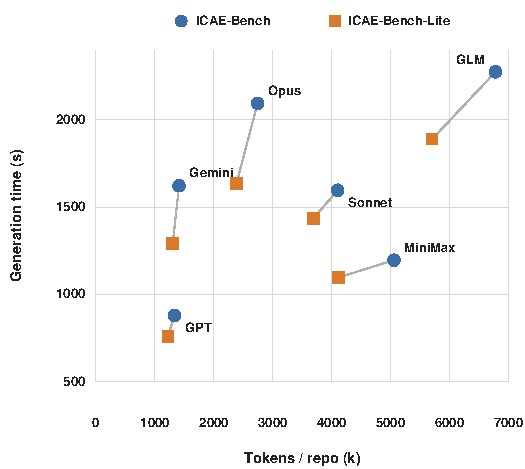
\includegraphics[width=\linewidth]{figures/runtime_token_scatter.pdf}
\caption{Runtime and token usage for main Claude Code runs on \rcb{} and \rcblite{}. Token counts are mean thousands of recorded tokens per repository; lines connect the same model across splits.}
\label{fig:runtime-cost}
\end{figure}

% \subsection{Implications.}
% Across RQ2--RQ4, access to more requirement information does not consistently yield more correct repositories. The strongest gains instead arise when information becomes actionable, as with executable Public cases. This pattern motivates agents that preserve clarified constraints, connect them to implementation decisions, and verify those decisions throughout repository construction.

% \subsection{Implications.}
% Across RQ2--RQ4, a consistent pattern emerges: access to more requirement information does not by itself produce better repositories. Gains are largest when the system makes information actionable through executable feedback or reliable framework support. Future coding agents should therefore preserve clarification as project state, connect recovered constraints to implementation and verification steps, and detect when later edits violate earlier decisions. ICAE-Bench evaluates this full process from requirement discovery to verified software, rather than clarification alone.
